\documentclass[11pt]{article} % Font size
%\usepackage[utf8]{inputenc}
%\usepackage{graphicx}
%\graphicspath{{Figures/}{./}}
%\usepackage[slovak]{babel}
%\usepackage{amsmath}
%%%%%%%%%%%%%%%%%%%%%%%%%%%%%%%%%%%%%%%%%
% Wenneker Assignment
% Structure Specification File
% Version 2.0 (12/1/2019)
%
% This template originates from:
% http://www.LaTeXTemplates.com
%
% Authors:
% Vel (vel@LaTeXTemplates.com)
% Frits Wenneker
%
% License:
% CC BY-NC-SA 3.0 (http://creativecommons.org/licenses/by-nc-sa/3.0/)
% 
%%%%%%%%%%%%%%%%%%%%%%%%%%%%%%%%%%%%%%%%%

%----------------------------------------------------------------------------------------
%	PACKAGES AND OTHER DOCUMENT CONFIGURATIONS
%----------------------------------------------------------------------------------------

\usepackage{amsmath, amsfonts, amsthm} % Math packages

\usepackage{listings} % Code listings, with syntax highlighting

\usepackage[slovak]{babel} % English language hyphenation

\usepackage{graphicx} % Required for inserting images
\graphicspath{{Figures/}{./}} % Specifies where to look for included images (trailing slash required)

\usepackage{booktabs} % Required for better horizontal rules in tables

\usepackage{caption}
\usepackage{subcaption}

\numberwithin{equation}{section} % Number equations within sections (i.e. 1.1, 1.2, 2.1, 2.2 instead of 1, 2, 3, 4)
\numberwithin{figure}{section} % Number figures within sections (i.e. 1.1, 1.2, 2.1, 2.2 instead of 1, 2, 3, 4)
\numberwithin{table}{section} % Number tables within sections (i.e. 1.1, 1.2, 2.1, 2.2 instead of 1, 2, 3, 4)

\setlength\parindent{0pt} % Removes all indentation from paragraphs

\usepackage{enumitem} % Required for list customisation
\setlist{noitemsep} % No spacing between list items

%----------------------------------------------------------------------------------------
%	DOCUMENT MARGINS
%----------------------------------------------------------------------------------------

\usepackage{geometry} % Required for adjusting page dimensions and margins

\geometry{
	paper=a4paper, % Paper size, change to letterpaper for US letter size
	top=2cm, % Top margin
	bottom=2cm, % Bottom margin
	left=2cm, % Left margin
	right=2cm, % Right margin
	headheight=0.75cm, % Header height
	footskip=1.5cm, % Space from the bottom margin to the baseline of the footer
	headsep=0.75cm, % Space from the top margin to the baseline of the header
	%showframe, % Uncomment to show how the type block is set on the page
}

%----------------------------------------------------------------------------------------
%	FONTS
%----------------------------------------------------------------------------------------

\usepackage[utf8]{inputenc} % Required for inputting international characters
\usepackage[T1]{fontenc} % Use 8-bit encoding

\usepackage{fourier} % Use the Adobe Utopia font for the document

%----------------------------------------------------------------------------------------
%	SECTION TITLES
%----------------------------------------------------------------------------------------

\usepackage{sectsty} % Allows customising section commands

\sectionfont{\vspace{6pt}\centering\normalfont\scshape} % \section{} styling
\subsectionfont{\normalfont\bfseries} % \subsection{} styling
\subsubsectionfont{\normalfont\itshape} % \subsubsection{} styling
\paragraphfont{\normalfont\scshape} % \paragraph{} styling

%----------------------------------------------------------------------------------------
%	HEADERS AND FOOTERS
%----------------------------------------------------------------------------------------

\usepackage{scrlayer-scrpage} % Required for customising headers and footers

\ohead*{} % Right header
\ihead*{} % Left header
\chead*{} % Centre header

\ofoot*{} % Right footer
\ifoot*{} % Left footer
\cfoot*{\pagemark} % Centre footer
 % Include the file specifying the document structure and custom commands

%----------------------------------------------------------------------------------------
%	TITLE SECTION
%----------------------------------------------------------------------------------------

\title{	
	\normalfont\normalsize
	\textsc{Slovenská technická univerzita v Bratislave, fakulta elektrotechniky a informatiky}\\ % Your university, school and/or department name(s)
	\vspace{25pt} % Whitespace
	%\rule{\linewidth}{0.5pt}\\ % Thin top horizontal rule
	\vspace{20pt} % Whitespace
	\vspace{20pt} % Whitespace
	\vspace{20pt} % Whitespace
	\vspace{20pt} % Whitespace
	\vspace{20pt} % Whitespace
	\vspace{20pt} % Whitespace
	\vspace{20pt} % Whitespace
	\vspace{20pt} % Whitespace
		\vspace{20pt} % Whitespace
	\vspace{20pt} % Whitespace
	\huge Simulátor diabetu\\ % The assignment title
	\vspace{12pt} % Whitespace
	\normalsize Biokybernetika, zadanie č.3
	\vspace{20pt} % Whitespace
	\vspace{20pt} % Whitespace
	\vspace{20pt} % Whitespace
		\vspace{20pt} % Whitespace
	\vspace{20pt} % Whitespace
		\vspace{20pt} % Whitespace
	\vspace{20pt} % Whitespace
		\vspace{20pt} % Whitespace
	\vspace{20pt} % Whitespace
	\vspace{20pt} % Whitespace
	\vspace{20pt} % Whitespace
		\vspace{20pt} % Whitespace
	\vspace{20pt} % Whitespace
	%\rule{\linewidth}{2pt}\\ % Thick bottom horizontal rule
	\vspace{12pt} % Whitespace
}

\author{\LARGE Lukáš Šníder} % Your name

\date{november 2020}
%\date{\normalsize\today} 

\begin{document}

\maketitle % Print the title
\thispagestyle{empty}
\clearpage
\setcounter{page}{1}
\pagenumbering{arabic} 
%----------------------------------------------------------------------------------------
%	FIGURE EXAMPLE
%----------------------------------------------------------------------------------------

%\section{Zostavenie simulačnej schémy podsystému pre vstrebávanie glukózy}

\section{Opis modelu podsystému vstrebávania glukózy}
Tento podsystém reprezentuje vstrebávanie glukózy z tráviaceho traktu do krvi a skladá sa z nasledovných rovníc:
\begin{eqnarray}
	\dot{D}(t) &=& -\left(\frac{1}{T_D}\right) D(t) + A_{G}d(t) \label{eq:pvg1} \\ 
	\dot{Ra}(t) &=& -\left(\frac{1}{T_D}\right) Ra(t) + \left(\frac{1}{T_D}\right) D(t) \label{eq:pvg2}
\end{eqnarray}

Vstupom tohto podsystému je rýchlosť prijímania sacharidov v čase \textit{d(t)} $[mg/kg/min]$, ide o impulz, ktorého šírka je rovná perióde vzorkovania a plocha je rovná množstvu prijatých sacharidov, parametrami sú: \textit{$T_D$ $[min]$}, čo je časová konštanta, \textit{$A_G$ $[bezrozmerné]$} je zlomok z prijatých sacharidov, ktoré sa efektívne vstrebú. Výstupom je signál \textit{Ra(t)} \textit{$[mg/kg/min]$}.

\section{Spracovanie a zobrazenie CGM dát}

V rámci týchto dát máme k dispozícií všetky vstupy potrebné na úspešné spustenie nášho simulátora. 

Sú medzi nimi tieto:
\begin{enumerate}
\item samotné údaje o CGM (angl. \textit{continuous glucose monitoring}) [min, mmol/l], sú zobrazené na obrázku ~\ref{fig:cgm_glykemia}
\item dáta z glykomera [min, mmol/l], majú informatívny charakter, taktiež ich možno vidieť na obrázku ~\ref{fig:cgm_glykemia}
\item jednorazové dávky sacharidov v sacharidových jednotkách [min, SJ] (1 [SJ] = 10 [g]), budú vstupom do podsystému vstrebávania glukózy \textit{d(t)}. Zo sacharidových jednotiek sme ich museli previesť do [mg/kg/min] prenásobením konštantou \[ \frac{\num{1e4}}{BW T_S} \] kde BW je telesná hmotnosť, ktorú sme uvažovali 64.6 [kg] (získané z údajov o celkovom boluse a podanom boluse v učebnom texte - 12,92[U]/0,2[U/kg]) a veľkosť $T_S$ uvažuje 1 [min]. Takto spracované dáta možno vidieť na \ref{fig:Ng1}.
\item bazálna rýchlosť podávania inzulínu [min, U/h], poslúži ako vstup do podsystému vstrebávania inzulínu $v_b$. Z jednotiek vo vstupnom súbore sme aj tieto dáta prevádzali do [mg/kg/min], prenásobením konštantou \[ \frac{\num{1e6}}{60 BW} \] pre BW = 64,6 [kg]. \footnote{V dátach sme mali ľahko identifikovateľnú chybu (nulovú hodnotú), spôsobenú zrejme chybou pri meraní, ktorú sme nahradili na hodnotu z okolitých meraní.}
\item údaje o podanom boluse [min, U], budú použité ako ďalší vstup do podsystému vstrebávania inzulínu $v_B$. Z jednotiek vo vstupnom súbore sme opäť dáta prevádzali do [mg/kg/min], tentokrát prenásobením konštantou \[ \frac{\num{1e6}}{BW} \] pre BW = 64,6 [kg]. Výsledné dáta $v_b$ a $v_B$ môžme vidieť spolu na \ref{fig:Ng2} v logarimickej mierke.
\end{enumerate}

\newpage

\begin{figure}[h] 
	\centering
	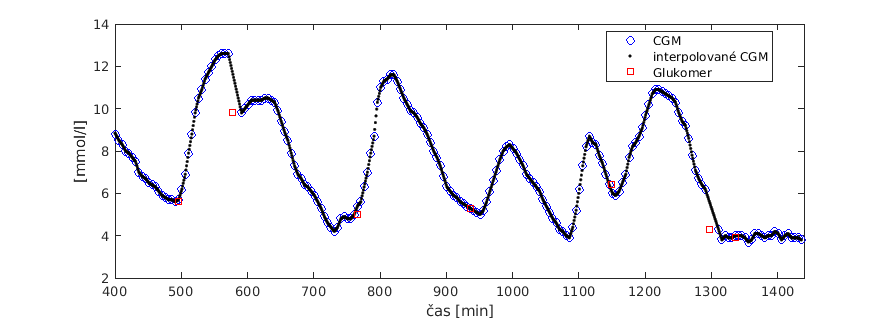
\includegraphics[width=1.0\columnwidth]{cgm_data.png} 
	\caption{Priebeh glykémie zo vstupných dát.}
	\label{fig:cgm_glykemia}
\end{figure}

\begin{figure}[h]
\centering
\begin{subfigure}[b]{0.7\textwidth}
   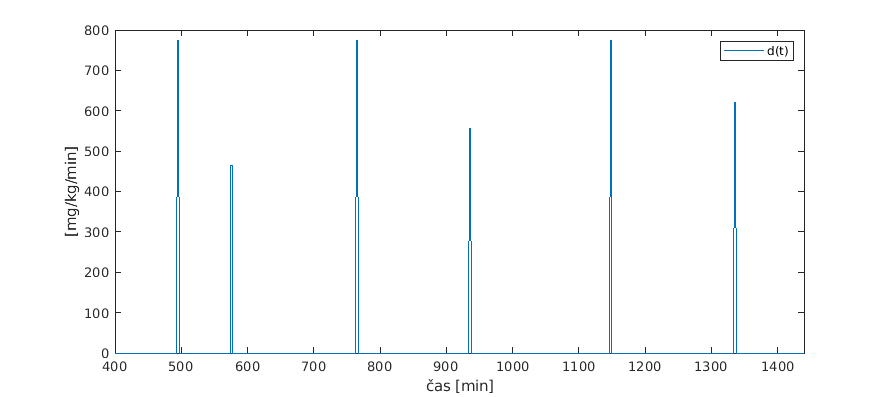
\includegraphics[width=1\linewidth]{podavanie_glukozy.png}
   \caption{}
   \label{fig:Ng1} 
\end{subfigure}

\begin{subfigure}[b]{0.7\textwidth}
   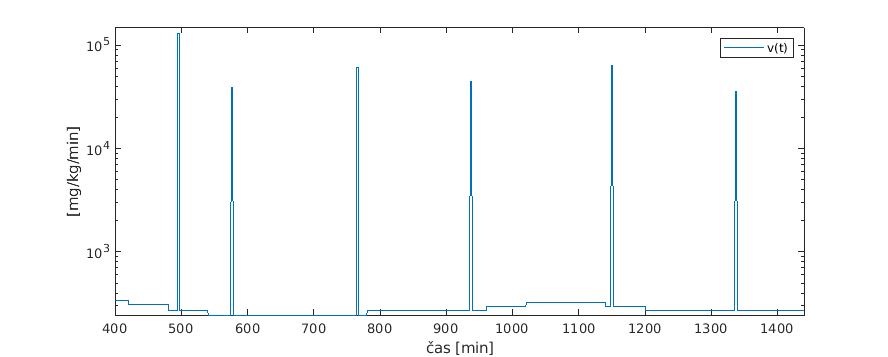
\includegraphics[width=1\linewidth]{podavanie_inzulinu.png}
   \caption{}
   \label{fig:Ng2}
\end{subfigure}
\caption[Two numerical solutions]{(a) Podávanie sacharidov podľa vstupných dát. 
(b) Rýchlosť podávania inzulínu.}
\end{figure}

\newpage

\section{Vzorová simulácia zostaveného simulátora}

\subsection{Podsystém vstrebávania glukózy}

Na nasledujúcom obrázku \ref{fig:schema_glukozy} je zobrazený podsystém pre vstrebávanie glukózy, zostavený podľa rovníc ~\ref{eq:pvg1} a \ref{eq:pvg2}.

\begin{figure}[h]
	\centering
	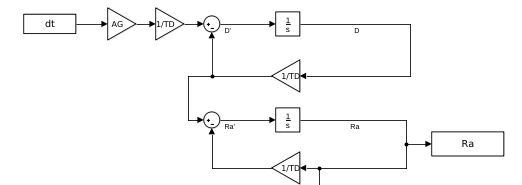
\includegraphics[width=0.9\columnwidth]{schema_podsystemu_vstrebavania_glukozy.png} 
	\caption{Schéma podsystému vstrebávania glukózy.}
	\label{fig:schema_glukozy}
\end{figure}

\subsection{Overovacia simulácia}

Pripravený podsystém môžme pridať do nášho simulatóra diabetu, ktorého celá schéma je na obrázku ~\ref{fig:cely_simulator}. Čo sa týka samotnej simulácie budeme používať parametre z učebného textu, ktoré slúžili na overenie ostatných podsystémov:
\begin{itemize}
\item $T_I$ = 44,55 [min]
\item $k_I$ = 0,1645 [1/min]
\item $V_I$ = 138,8 [dl/kg]
\item $S_I$ = 0,0159 [ml/$\mu$ U/min]
\item $p_2$ = 0,0106 [1/min]
\end{itemize}
rovnako ako ďalšie už použité parametre, t.j. $G_B$ = 153 [mg/dl], $V_G$ = 1,467 [dl/kg] a pridaný parameter $A_G$ = 0,95 volíme opäť podľa učebného textu. Parametre, ktoré overujeme sú:
\begin{itemize}
\item $S_G = 0,032$ [1/min]
\item $T_D = 33,474$ [min]
\end{itemize}

Na obrázku ~\ref{fig:vystup_glukozy} môžme vidieť výstup tohto podsystému $Ra(t)$ porovnamý so vstupným signálom $d(t)$. 

%\begin{figure}[h]
%	\centering
%	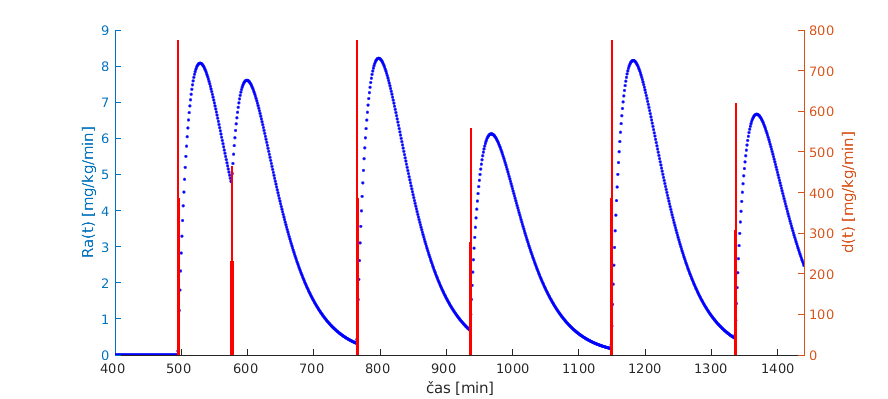
\includegraphics[width=0.9\columnwidth]{Ra_vystup.png} 
%	\caption{Rýchlosti vstrebávania glukózy a podávania sacharidov.}
%	\label{fig:vystup_glukozy}
%\end{figure}

Zvyšná časť simulátora pozostáva z podsystému vstrebávania inzulínu, 
na \ref{fig:vystup_inzulin} môžme vidieť koncentráciu inzulínu $I(t)$ a rýchlosť jeho podávania $v(t)$
a Bergmanovho minimálneho modelu, pre reguláciu koncentrácie glukózy v krvi.

\begin{figure}[!htb]
	\centering
	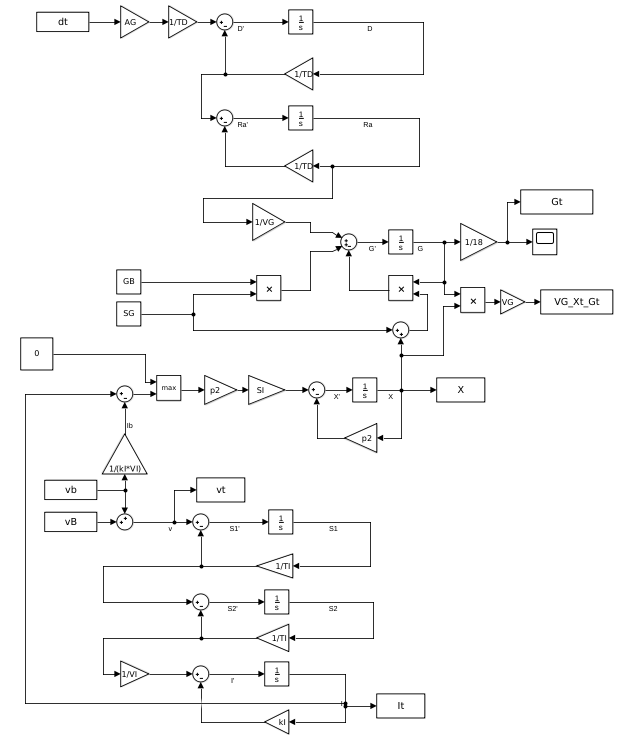
\includegraphics[width=1.0\columnwidth]{schema_simulator_diabetu.png} 
	\caption{Schéma simulátora diabetu.}
	\label{fig:cely_simulator}
\end{figure}

\newpage

Výslednú hladinu glykémie je možné vidieť na obrázku \ref{fig:simulator_vystup}. Simuláciu sme začínali až od 400-tej minúty poskytnutých vstupných dát, kedže až niečo pred 500-tou minútou dochádza k prijmu sacharidov, ako aj bolusovej dávky inzulínu, čo je práve pre nás zaujímavé, z podobného dôvodu nulujeme záporné hodnoty signálu $I(t)$, (po odpočítaní $I_b$), ktorý vstupuje do Bermanovho minimálneho modelu, keďže záporné hodnoty ako výstup podsystému vstrebávania inzulínu nedávajú zmysel. Táto situácia nastáva na začiatku simulácie.  

\begin{figure}[!htb]
	\centering
	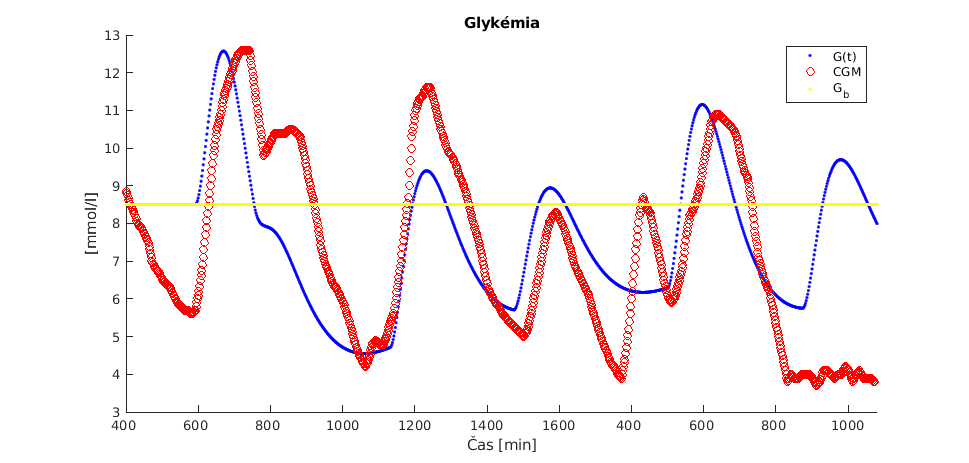
\includegraphics[width=1.0\columnwidth]{simulator_vystup.png} 
	\caption{Hladina glykémie počas simulácie.}
	\label{fig:simulator_vystup}
\end{figure}

\begin{figure}[h]
	\centering
	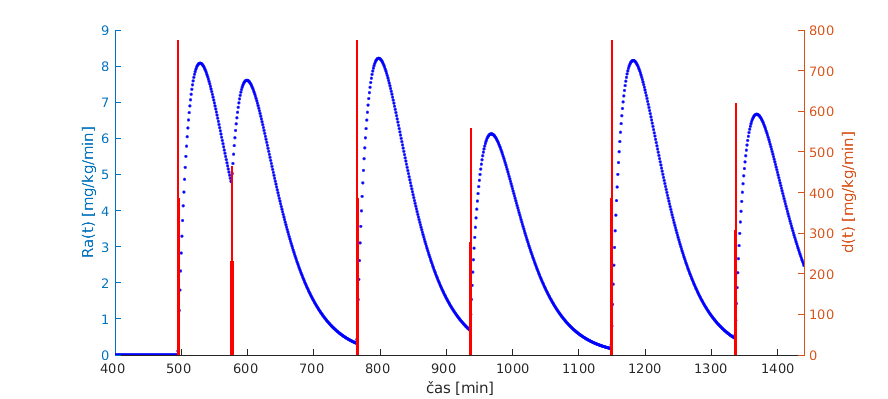
\includegraphics[width=0.9\columnwidth]{Ra_vystup.png} 
	\caption{Rýchlosti vstrebávania glukózy a podávania sacharidov.}
	\label{fig:vystup_glukozy}
\end{figure}

\begin{figure}[h]
	\centering
	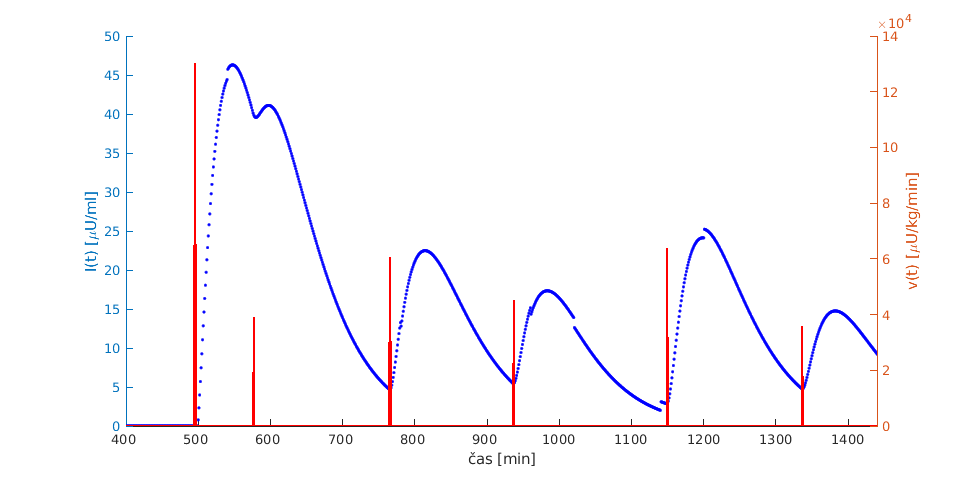
\includegraphics[width=0.9\columnwidth]{inzulin_vzor.png} 
	\caption{Koncentrácia inzulínu a rýchlosť podávania inzulínu.}
	\label{fig:vystup_inzulin}
\end{figure}


\newpage

\section{Identifikácia parametrov podsystému vstrebávania glukózy}
Parametre na identifikáciu:
\begin{itemize}
\item $S_G$ [1/min]
\item $T_D$ [min]
\end{itemize}

Pri identifikácií budeme požívať vlastné parametre, teda $T_I$ = 42,8216 [min], $k_I$ = 0,1939 [1/min], $V_I$ = 110,5990 [dl/kg], $S_I$ = 0,0014 [ml/$\mu$ U/min], $p_2$ = 0,0097 [1/min] a rozhodli sme sa opäť použiť genetický algoritmus. Pre účely tejto úlohy si z hľadaných parametrov vyskladáme chromozóny jedincov, ktoré budú vystupovať v evolúcií nášho genetického algoritmu, takže každý jedinec bude pozostávať z dvoch génov $S_G$, $T_D$.

Na začiatku je dôležité vhodne si zadefinovať stavový priestor prehľadávania, t.j. horné a dolné ohraničenie pre jednotlivé parametre. Pri ich nesprávnom nastavení sa môže stať, že sa nám nepodarí nájsť dostatočne dobré riešenie, po niekoľkých testoch sme sa dostali k nasledovným ohraničeniam: 
\[ 0,0001 < S_G < 0,1, \hspace{3mm} 0,1 < T_D < 200, \] 
V rámci samotného algoritmu sme sa snažili zvoliť stredne veľký selektívny tlak a stredne veľkú diverzitu, takže sme vyberali do ďalšej generácie 10\% najlepších jedincov z aktuálnej populácie a pre zvyšok sme volili mutácie na úrovni 20\%. Dĺžku evolúcie sme nastavili na 30 generácií a jej priebeh je na obrázku \ref{fig:evolution}.

\begin{figure}[!htb]
	\centering
	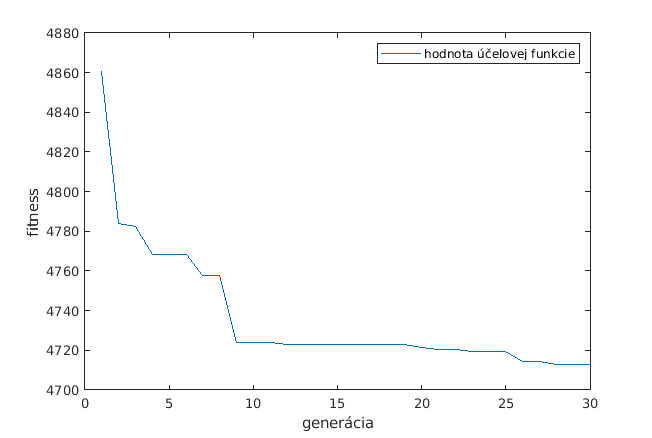
\includegraphics[width=0.7\columnwidth]{evolution.png} 
	\caption{Vývoj evolúcie účelovej funkcie.}
	\label{fig:evolution}
\end{figure}

Pri tvorbe samotnej účelovej funkcie sme vychádzali z učebného textu a použili nasledovnú:

\begin{equation}
 min \hspace{5mm} \| y - \hat{y}(\theta_3) \|^2 \hspace{2mm}  
\end{equation}

odtiaľ $y$ je vektor hodnôt vstupných CGM dát a $\hat{y}$  je vektor výstupných hodnôt glykémie našej simulácie pre parametre $\theta_3 = [S_G  T_D]$. Touto funkciou si problém formulujeme ako úlohu nelineárnej metódy najmenších štvorcov a snažíme sa v nej minimalizovať odchýlky od nameraných CGM dát. 

Nakoniec sa nám týmto postupom podarilo identifikovať nasledujúce parametre:
\begin{itemize}
\item $S_G = 0,0159 \hspace{1mm}[1/min]$ 
\item $T_D = 41,1727 \hspace{1mm}[min]$ 
\end{itemize}

Na obrázku ~\ref{fig:identifikacia_vystup} je priebeh hladiny glykémie po aplikovaní našich parametrov do simulácie, na obrázkoch \ref{fig:Ra_vlastny} a ~\ref{fig:inzulin_vlastny} výstupy podsystémov pre vstrebávanie glukózy a vstrebávanie inzulínu.
 

\begin{figure}[!htb]
	\centering
	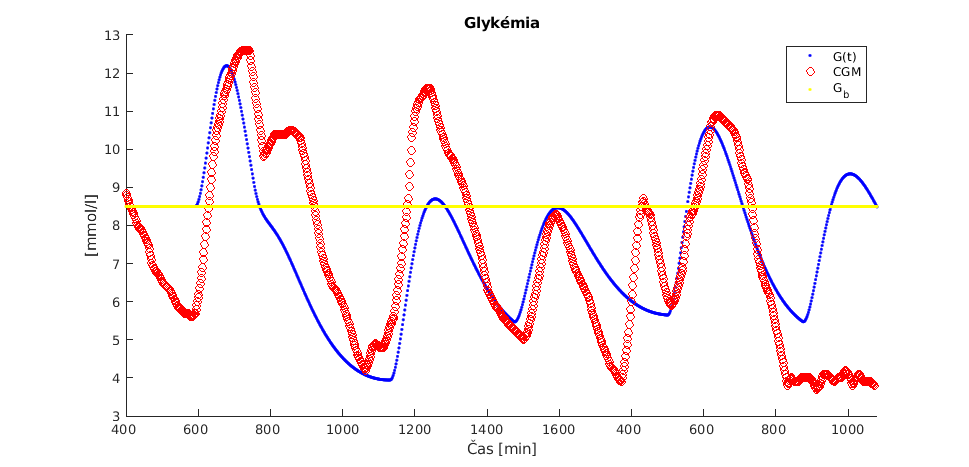
\includegraphics[width=0.9\columnwidth]{identifikacia_vystup.png} 
	\caption{Hladina glykémie počas simulácie s nami definovanými parametrami.}
	\label{fig:identifikacia_vystup}
\end{figure}

\begin{figure}[!htb]
	\centering
	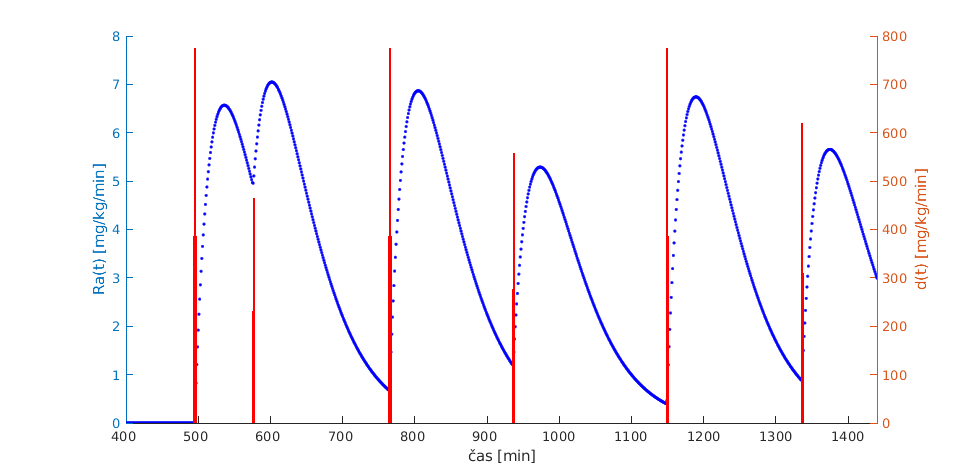
\includegraphics[width=0.9\columnwidth]{Ra_vlastny.png} 
	\caption{Rýchlosti vstrebávania glukózy a podávania sacharidov.}
	\label{fig:Ra_vlastny}
\end{figure}


\begin{figure}[!htb]
	\centering
	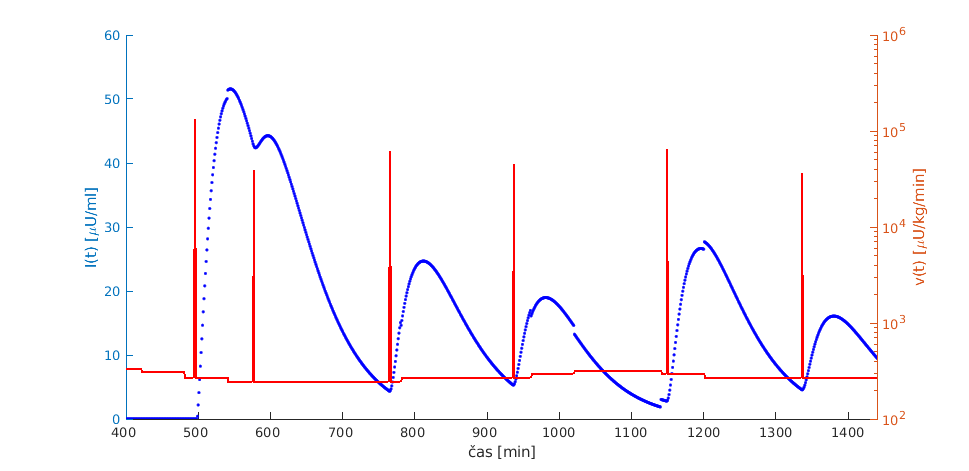
\includegraphics[width=0.9\columnwidth]{inzulin_vlastny.png} 
	\caption{Koncentrácia inzulínu a rýchlosť podávania inzulínu.}
	\label{fig:inzulin_vlastny}
\end{figure}


\section{Vyhodnotenie výsledkov identifikácie}
V práci sme sa snažili namodelovať simulátor diabetu, pre prípad, že máme k dispozícií CGM dáta ako želané výstupné hodnoty nášho modelu, vstupné dáta o prijímaných sacharidoch a dáta s rýchlosťou podávania inzulínu. 

S týmito dátami a naším simulátorom sa snažíme modelovať procesy regulovania glykémie v krvi v situácií, keď subjekt, o ktorom tieto dáta máme, prijal v strave zadané množstvo sacharidov, ktoré sú v našich vstupných dátach uvedené a zároveň mu bol do podkožia v rovnakom čase podávaný inzulín, v množstvách, ktoré sú opäť v dostupných dátach. Tieto informácie používame ako vstupy do nášho modelu, ktorý sme identifikovali na základe CGM dát, ktoré sú želanými výstupnými hodnotami. Na účely identifikácie sme použili genetický algoritmus a minimalizovali sme odchýlky štvorcov výstupu nášho modelu a CGM dát. Týmto postupom sme sa dopracovali k posledným dvom parametrom, t.j. $S_G$ = 0,0159 [l/min] a  $T_D$ = 41,1727 [min], potrebným na finalizáciu nášho simulátora diabetu.

Keďže vo výstupnom signále modelu po odsimulovaní s použitím vyššie spomenutých vstupných dát je vidieť kopírovanie hodnôt z CGM dát, môžme povedať, že sa nám podarilo navrhnúť systém, ktorý možno použiť ako prispôsobiteľný simulátor diabetu. 

\vspace{5mm}

Zhrnutie identifikovaných parametrov:
\begin{itemize}
\item $T_I$ = 42,8216 [min]
\item $k_I$ = 0,1939 [1/min]
\item $V_I$ = 110,5990 [dl/kg]
\item $S_I$ = 0,0014 [ml/$\mu$ U/min]
\item $p_2$ = 0,0097 [1/min]
\item $S_G$ = 0,0159 [l/min]
\item $T_D$ = 41,1727 [min]
\end{itemize}

\end{document}
